% ==============================================================================
% EXPERIMENTOS
% ==============================================================================
% Instrucciones de la plantilla:
% - Detallar de manera clara y estructurada las pruebas realizadas.
% - Incluir tanto los resultados exitosos como los fallidos.
% - Detallar las variaciones exploradas en cada actividad.
% - Describir los experimentos base: objetivo, metodología empleada y resultados obtenidos.
% ==============================================================================

\section{Experimentos}

En esta sección se describen las pruebas que hicimos en cada actividad, incluidas las que fallaron, porque varias de las decisiones de la metodología salieron precisamente de esas fallas.

% ------------------------------------------------------------------------------
\subsection{Experimentos de la Actividad 1: canal alfa de la hoja}

\subsubsection{Objetivo del experimento}
Obtener una textura RGBA de la hoja a partir de una fotografía que no trae canal alfa, y comprobar que la transparencia se conserva desde Blender hasta OpenGL.

\subsubsection{Pruebas fallidas y análisis de errores}
\textbf{Máscara elíptica.} Como la hoja tiene forma casi elíptica, la primera versión del alfa fue una elipse con borde suave ajustada a mano, con centro $(371, 364)$ y semiejes $223 \times 242$. Al componer el resultado sobre magenta (Figura \ref{fig:mascaras}, izquierda) aparecieron dos defectos: la punta superior de la hoja es más angosta que la elipse, así que se coló fondo arriba a la izquierda, y en la parte de abajo quedó visible la yema del pulgar.

\textbf{Umbral de color.} La segunda versión separó la hoja por su color y se quedó con la región conectada al centro (Figura \ref{fig:mascaras}, centro). La orilla quedó mucho más fiel, pero con tres defectos nuevos: la punta superior, más clara que el resto, no pasó el umbral; dos manchas del fondo del mismo naranja quedaron pegadas a los costados, y apareció un hueco abajo a la izquierda.

La versión final combina las dos ideas: el umbral de color da la orilla y la elipse, agrandada un 4\,\%, sirve solo como límite para cortar las manchas; el relleno por filas recupera la punta y los huecos (Figura \ref{fig:mascaras}, derecha).

\begin{figure}[H]
    \centering
    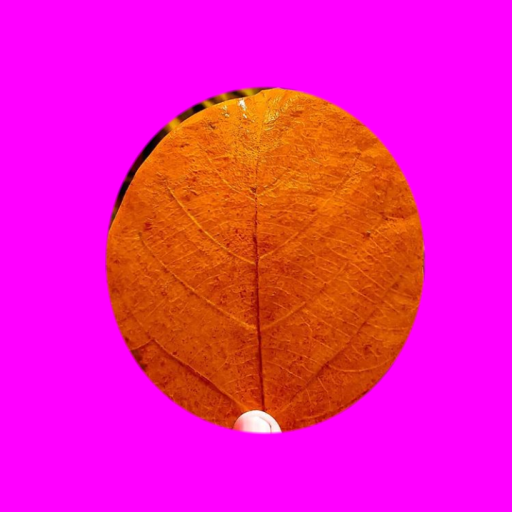
\includegraphics[width=0.31\textwidth]{Imagenes/E1/04_mascara_elipse.png}
    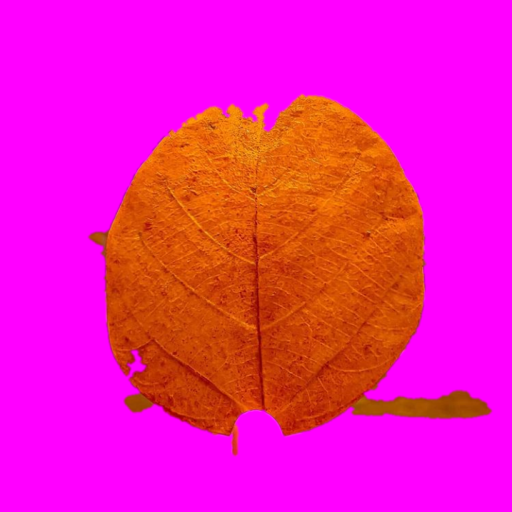
\includegraphics[width=0.31\textwidth]{Imagenes/E1/05_mascara_color.png}
    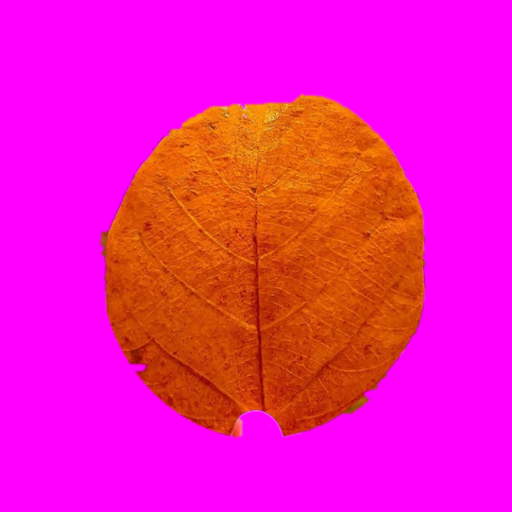
\includegraphics[width=0.31\textwidth]{Imagenes/E1/02_hoja_rgba_magenta.png}
    \caption{Tres versiones del canal alfa compuestas sobre magenta: elipse ajustada a mano (izquierda), umbral de color con región conexa (centro) y combinación final con límite elíptico y relleno por filas (derecha).}
    \label{fig:mascaras}
\end{figure}

\textbf{Un falso negativo en la verificación.} Al revisar la primera textura con un guion auxiliar, este reportó que el alfa valía 1 en todos los píxeles, como si la máscara no se hubiera guardado. Antes de cambiar el código que la generaba comprobamos por separado la escritura y la lectura del PNG, y las dos eran correctas: el error estaba en el guion de verificación, que imprimía el alfa de una \textit{vista} del arreglo de NumPy después de haberlo sobrescrito con 1. La textura siempre había estado bien.

\textbf{El nombre del nodo.} El guion funcionó en la prueba sin interfaz, pero al ejecutarlo con Blender abierto falló al buscar el nodo con \texttt{nodes.get("Principled BSDF")}: la interfaz de Blender está en español y el nodo se llama de otra forma. Desde entonces los nodos se buscan por su tipo, \texttt{BSDF\_PRINCIPLED}, que no depende del idioma.

\subsubsection{Pruebas exitosas}
Cargada en OpenGL, la hoja se dibuja con su contorno recortado y el pasto del fondo se ve alrededor (Figura \ref{fig:opengl_hoja}), lo que confirma que el canal alfa llega intacto hasta el \textit{shader} a través de Assimp y \texttt{stb\_image}: \texttt{TextureFromFile} detecta los 4 canales del PNG y sube la imagen como \texttt{GL\_RGBA}.

% ------------------------------------------------------------------------------
\subsection{Experimentos de la Actividad 2: posición de la caja}

\subsubsection{Objetivo del experimento}
Verificar que varias figuras exportadas en un mismo FBX conservan en OpenGL la posición que tienen en Blender.

\subsubsection{Pruebas fallidas y análisis de errores}
Al exportar la hoja y la caja juntas, la caja apareció en el centro de la escena y la hoja desapareció (Figura \ref{fig:caja_centrada}). En Blender la caja está en $x = 3$, pero el exportador guarda esa posición en la matriz del nodo y deja los vértices en coordenadas locales, alrededor del origen. Revisando \texttt{model.h} confirmamos que \texttt{processNode} recorre los nodos sin aplicar nunca \texttt{mTransformation}, así que todas las mallas se dibujan en su espacio local: la caja, de 2 unidades por lado, quedó centrada en el origen y la hoja, que está en $z = 0$, quedó dentro de ella.

\begin{figure}[H]
    \centering
    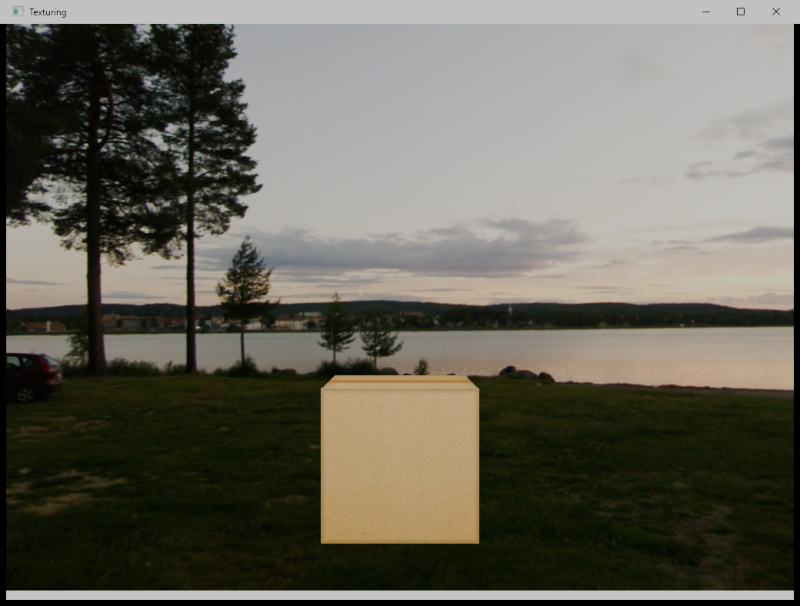
\includegraphics[width=0.55\textwidth]{Imagenes/E2/03_opengl_caja_centrada.png}
    \caption{Primera exportación de la hoja y la caja: la caja se dibuja en el origen, ignorando su posición, y oculta a la hoja.}
    \label{fig:caja_centrada}
\end{figure}

Había dos soluciones: aplicar las transformaciones en Blender (\textit{Ctrl+A}) o hacerlo solo en el archivo exportado. Elegimos la segunda, con las copias temporales del Listado \ref{lst:exportar}, porque la primera mueve el origen de cada objeto al origen del mundo y ya no se puede reacomodar la escena con comodidad.

\subsubsection{Pruebas exitosas}
Con la exportación corregida, la caja aparece a la derecha de la hoja y las dos se ven completas (Figura \ref{fig:caja_hoja}).

\begin{figure}[H]
    \centering
    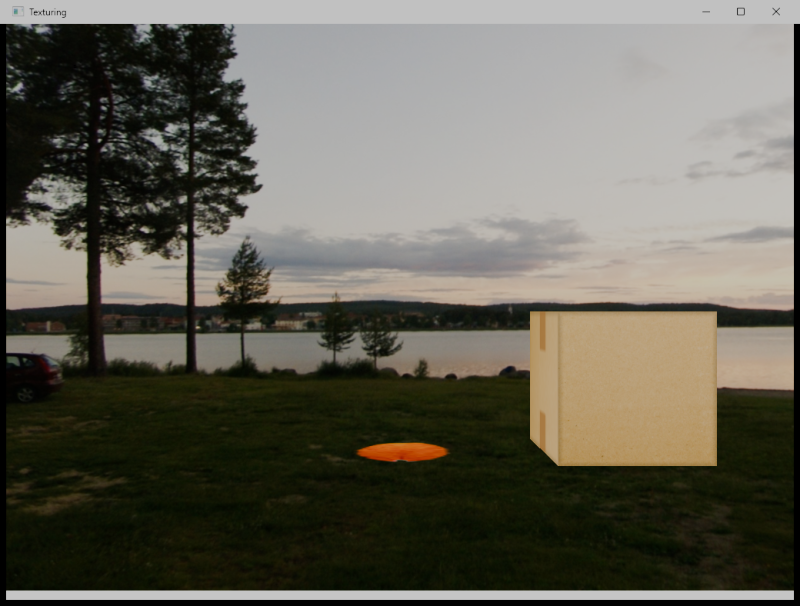
\includegraphics[width=0.55\textwidth]{Imagenes/E2/04_opengl_caja_hoja.png}
    \caption{Hoja y caja en sus posiciones después de exportar las mallas con la transformación aplicada.}
    \label{fig:caja_hoja}
\end{figure}

% ------------------------------------------------------------------------------
\subsection{Experimentos de la Actividad 3: texturas y forma del barril}

\subsubsection{Objetivo del experimento}
Elegir las imágenes que mejor representan un barril y comprobar que la edición proporcional produce la forma abombada sin alterar las tapas.

\subsubsection{Pruebas exitosas}
Comparamos tres texturas de madera y cuatro de metal (Figura \ref{fig:candidatas}). De las maderas descartamos \texttt{Planks012} y \texttt{Planks020} para las duelas porque son pisos de tablas cortas con juntas a tope, que en el costado del barril se verían como duelas partidas; \texttt{Planks012} sí se usó en las tapas, donde las tablas cortas no estorban. De los metales escogimos \texttt{Metal021}, acero gris azulado con puntos de óxido, porque contrasta con la madera clara; \texttt{Metal011} se reservó para la reja.

\begin{figure}[H]
    \centering
    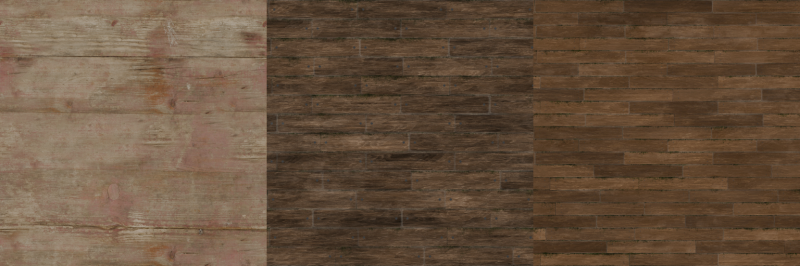
\includegraphics[width=0.75\textwidth]{Imagenes/E3/02_maderas_candidatas.png}\\[0.2cm]
    
\includegraphics[width=0.75\textwidth]{Imagenes/E3/02b_metales_candidatos.png}
    \caption{Texturas candidatas de ambientCG. Arriba, de izquierda a derecha: \texttt{Planks005}, \texttt{Planks012} y \texttt{Planks020}. Abajo: \texttt{Metal011}, \texttt{Metal021}, \texttt{Metal026} y \texttt{Metal036}.}
    \label{fig:candidatas}
\end{figure}

Para verificar la edición proporcional medimos el radio de los anillos después de escalar: 1.0 en los anillos de las tapas y 1.18 en el central, como se buscaba. La Figura \ref{fig:barril_antes_despues} compara el barril antes y después en OpenGL; los aros siguen la curva porque la subdivisión interpoló las coordenadas UV.

\begin{figure}[H]
    \centering
    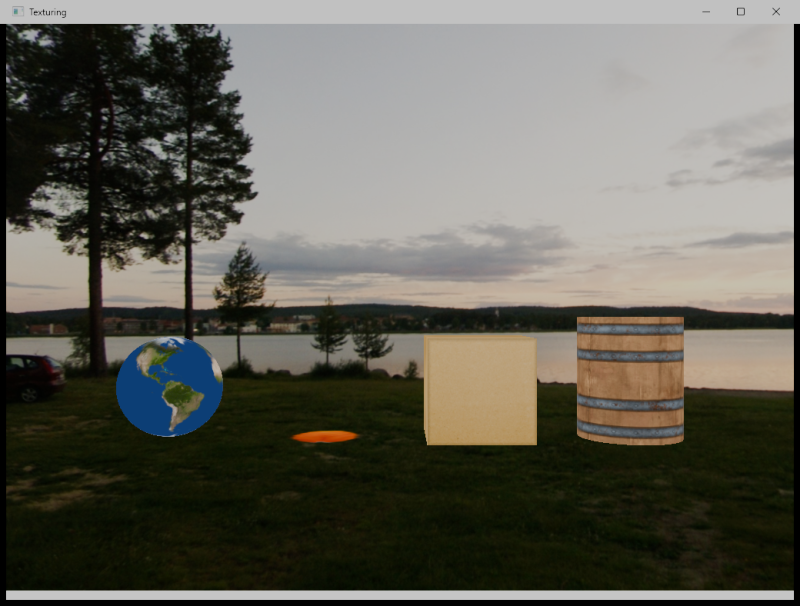
\includegraphics[width=0.48\textwidth]{Imagenes/E3/05_opengl_barril_cilindro.png}
    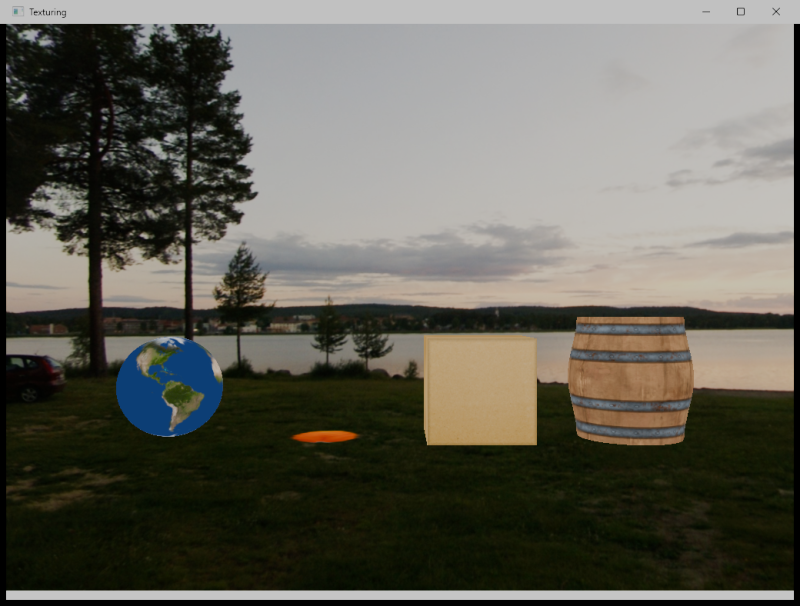
\includegraphics[width=0.48\textwidth]{Imagenes/E3/06_opengl_barril_forma.png}
    \caption{El barril en OpenGL como cilindro recto (izquierda) y después de la edición proporcional (derecha).}
    \label{fig:barril_antes_despues}
\end{figure}

% ------------------------------------------------------------------------------
\subsection{Experimentos de la Actividad 4: la esfera sin normales}

\subsubsection{Objetivo del experimento}
Cargar la esfera texturizada junto con las figuras anteriores y comprobar que la textura equirrectangular se ve sin deformaciones.

\subsubsection{Pruebas fallidas y análisis de errores}
\textbf{Cierre del programa.} Al agregar la esfera al FBX, el programa mostraba la ventana en negro y se cerraba (Figura \ref{fig:falla_normales}). El código de salida era \texttt{0xC0000005}, una violación de acceso, y el visor de eventos de Windows indicaba que ocurría dentro del propio \texttt{Proyecto06.exe}. Lo ejecutamos con el depurador de Visual Studio y la pila de llamadas lo ubicó en \texttt{Model::processMesh}, en la línea 173 de \texttt{model.h}, que lee \texttt{mesh->mNormals[i]}. Al inspeccionar las variables encontramos que Assimp entregaba la esfera (\texttt{Esfera.001}, con 8\,064 vértices y 3\,968 triángulos) con \texttt{mNormals} y \texttt{mTangents} en \texttt{NULL}: la esfera es la única malla con sombreado suave, y sus normales no llegaban en la forma en que Assimp las lee, mientras que las de la caja y el plano sí. El cargador del laboratorio da por hecho que toda malla trae normales y las lee sin revisar.

\begin{figure}[H]
    \centering
    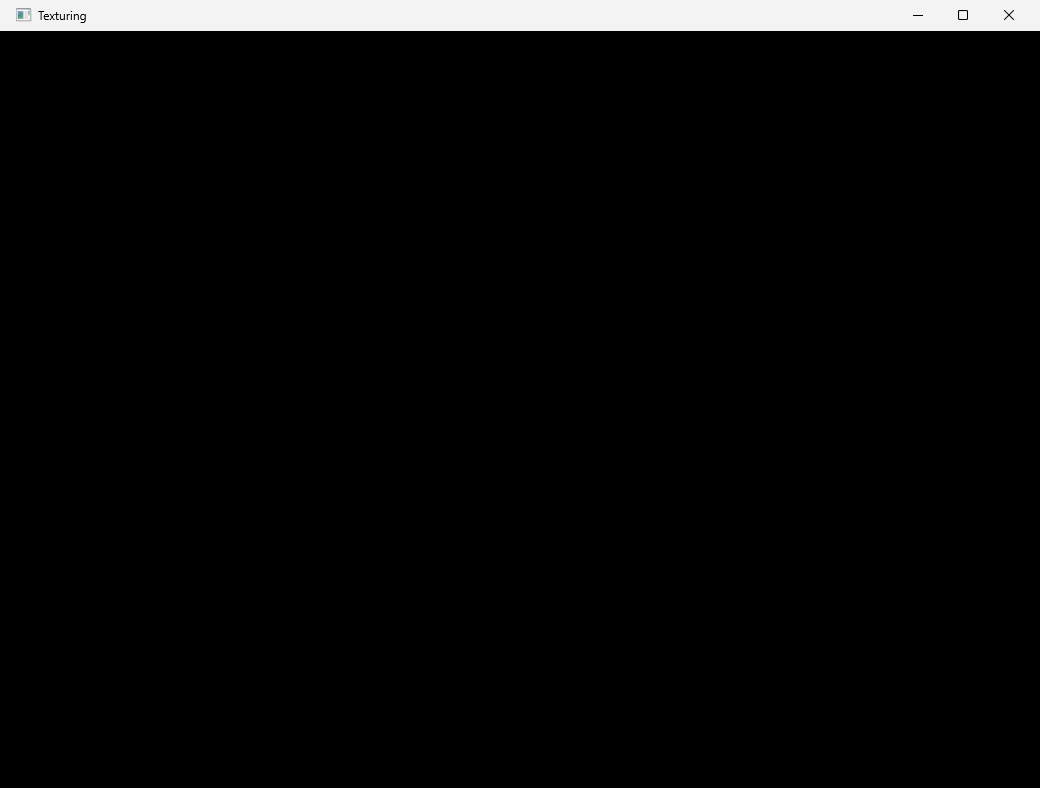
\includegraphics[width=0.32\textwidth]{Imagenes/E4/03_opengl_falla_normales.png}
    \caption{Ventana del programa al cargar la escena con la esfera, antes de cerrarse con la violación de acceso \texttt{0xC0000005}.}
    \label{fig:falla_normales}
\end{figure}

La corrección fue agregar \texttt{aiProcess\_GenSmoothNormals} a las banderas de \texttt{ReadFile}. Esa etapa de Assimp calcula normales suaves únicamente para las mallas que no las traen, así que no altera la caja ni el plano, y como corre antes de \texttt{aiProcess\_CalcTangentSpace}, las tangentes también quedan calculadas.

\textbf{La caja borrada.} El primer intento de crear la esfera falló dentro de Blender porque el operador \texttt{shade\_smooth} no tiene contexto cuando se ejecuta desde un temporizador. Al repetir el guion, este borró el objeto llamado «Planeta» antes de crear uno nuevo, y el objeto que se llevó fue la caja: en el primer intento el guion había tomado el objeto recién creado como \texttt{bpy.context.active\_object}, que dentro de un temporizador todavía apuntaba a la caja, y la había renombrado. Lo detectamos porque la exportación siguiente listó solo dos mallas. Desde entonces los guiones identifican el objeto nuevo comparando el conjunto de objetos antes y después de crearlo, y el sombreado suave se aplica con \texttt{mesh.shade\_smooth()}, que no depende del contexto. La caja se volvió a generar con su guion.

\subsubsection{Pruebas exitosas}
Con la corrección, la Tierra se ve con los continentes en su posición y sin deformaciones cerca del ecuador ni de los polos, y América no aparece espejeada, lo que confirma que la orientación del $u$ de la esfera UV de Blender coincide con la del mapa.

% ------------------------------------------------------------------------------
\subsection{Experimentos de la Actividad 5: dimensiones de las texturas}

\subsubsection{Objetivo del experimento}
Asegurar que todas las texturas que carga OpenGL midan potencias de dos.

\subsubsection{Pruebas fallidas y análisis de errores}
Las dos primeras texturas no cumplían: la hoja medía $717 \times 717$, por el recorte cuadrado de la foto, y el atlas de la caja $1536 \times 1536$, porque estaba organizado en una cuadrícula de $3 \times 3$ celdas de 512. La hoja se escaló a $1024 \times 1024$ después de calcular su alfa y el atlas pasó a una cuadrícula de $4 \times 4$, que con las mismas celdas de 512 da $2048 \times 2048$; las coordenadas UV se dividen ahora entre 4 en lugar de entre 3. Para comprobarlo no confiamos en Blender: leímos el ancho y el alto directamente del encabezado de cada PNG y JPG que quedó en \texttt{bin/models}.

% ------------------------------------------------------------------------------
\subsection{Experimentos de la Actividad 6: origen del mapa de entorno}

\subsubsection{Objetivo del experimento}
Sustituir el fondo sin modificar el modelo del cubo de entorno ni las imágenes que usan las demás prácticas.

\subsubsection{Pruebas exitosas}
Al copiar \texttt{mycube.fbx} a su propia carpeta junto con una carpeta \texttt{mycube.fbm} con las seis caras de \textit{Footballfield}, el programa cargó el nuevo fondo a la primera, y las caras quedaron en su lugar: el cielo arriba, el pasto abajo y el horizonte continuo entre las cuatro caras laterales. Esto confirma que el cubo del laboratorio fue armado con la misma convención de nombres que usa Humus (\texttt{posx} a \texttt{negz}).

% ------------------------------------------------------------------------------
\subsection{Experimentos de las variaciones}

\subsubsection{Objetivo del experimento}
Comprobar que las técnicas de las cuatro actividades se generalizan a objetos distintos y que las texturas calculadas (la malla de la reja y el patrón del balón) son correctas.

\subsubsection{Pruebas fallidas y análisis de errores}
\textbf{Hexágonos desalineados.} La primera textura del balón tenía unos pentágonos deformes, rodeados por hexágonos enormes (Figura \ref{fig:balon_error}, izquierda). Para revisarla no bastaba con la imagen equirrectangular, que deforma los polos, así que dibujamos el patrón visto de frente en proyección ortográfica. El producto punto entre los centros vecinos dio la pista: entre pentágonos valía 0.4472, el valor correcto del icosaedro, pero los centros de hexágono de la forma $(0, \pm 1/\varphi, \pm\varphi)$ no formaban el dodecaedro dual de \emph{ese} icosaedro, sino uno girado. El dual correcto tiene los vértices en $(\pm 1/\varphi, 0, \pm\varphi)$ y sus permutaciones cíclicas; con ese cambio el patrón quedó como el de un balón real (Figura \ref{fig:balon_error}, derecha).

\begin{figure}[H]
    \centering
    
\includegraphics[width=0.32\textwidth]{Imagenes/V/04c_balon_error.png}
    \hspace{0.05\textwidth}
    
\includegraphics[width=0.32\textwidth]{Imagenes/V/04b_balon_frente.png}
    \caption{Patrón del balón visto de frente: con el dodecaedro girado (izquierda) y con el dodecaedro dual correcto (derecha).}
    \label{fig:balon_error}
\end{figure}

\textbf{Tinaco demasiado oscuro.} La foto \texttt{Plastic006} es casi negra, y en la primera versión las estrías del tinaco no se distinguían. Se aclaró la base ($0.07 + 1.8\,c$) y se cambió la modulación de las estrías por $\cos^8$, que deja franjas angostas y marcadas en lugar de una variación suave.

\subsubsection{Pruebas exitosas}
La reja se dibuja delante del edificio y, a través de sus rombos, se ve completa la fachada que está detrás. Esto depende del descarte de fragmentos del Listado \ref{lst:shader_alpha}: el orden de dibujo de las ocho mallas dentro del modelo lo decide el FBX y no el programa, así que dibujar «primero lo opaco» no se puede garantizar, y sin el descarte los píxeles transparentes de la reja escribirían su profundidad y ocultarían lo que se dibujara después detrás de ella. Por la misma razón, el edificio se ve a través de los huecos de la reja sin importar desde qué lado se mire.
